\chapter{Diseño}
\label{cap:capitulo4}

\begin{flushright}
\begin{minipage}[]{9cm}
\emph{El diseño no es solo lo que se ve y lo que se siente. El diseño es cómo funciona}\\
\end{minipage}\\

Steve Jobs, \textit{conferencia de lanzamiento del Apple iPod, 2001}\\
\end{flushright}

\vspace{1cm}

Después de definir la plataforma de desarrollo, se procede a explicar el diseño de la aplicación.

El proyecto se divide en cuatro scripts, el primero se utiliza para crear o registrar un paciente, el segundo lanza la GUI y controla los parámetros del juego, el tercero permite visualizar el comportamiento del paciente durante la terapia, y el cuarto es el propio juego.

\section{Registro de un paciente}

Este script permite gestionar un conjunto de datos, que identifican a un paciente, mediante una GUI.

En primer lugar, se importan las bibliotecas estádar, mencionadas en el capítulo anterior, como \textit{tkinter}, que se utiliza para crear la interfaz gráfica, \textit{csv} para guardar los datos en un archivo .csv para su posterior uso, y \textit{os} para interactuar con el sistema de archivos.

Se obtiene el directorio de inicio del usuario y se crea un directorio dentro de este, si no existe, bajo el nombre \textit{database}, donde se almacenan los ficheros con los datos de registro y análisis terapéuticos de cada paciente.

Después, se crea una ventana principal con un título y tamaño fijo. Los datos se ingresan de forma ordenada a través de entradas de texto y hacen referencia al nombre, apellido e ID del paciente, frecuencia, amplitud y perturbación de la señal que generará el brazo robótico al inicio de la terapia, nivel y progreso del juego y un espacio para que el doctor incluya alguna observación.

Se valida que el ID sea un número, si no lo es, muestra un mensaje de advertencia.
Para guardar los datos se debe pulsar el botón \textit{Save} y para salir de la interfaz \textit{Exit}.
Los datos se guardan en un fichero .csv dentro de un subdirectorio bajo el nombre del ID. Si el archivo existe, se añaden los datos al final, si no, se crea.
Una vez los datos se han guardado, se muestra un mensaje de confirmación y se limpian los campos.
Es obligatorio especificar el ID en todos los casos, los campos restantes pueden dejarse en blanco.

En el Código \ref{cod:codejemplo}, escrito en \texttt{Python}, se muestra cómo se gestionan los directorios y la escritura del archivo .csv.

\begin{code}[h]
\begin{lstlisting}[language=Python]
def savedata():
    ID_DIR = os.path.join(DATABASE_DIR, id)
    os.makedirs(ID_DIR, exist_ok=True)
    file_name = f"{id}{ext}"
    file_path = os.path.join(ID_DIR, file_name)

    # [...]

    file_exists = os.path.isfile(file_path)
    with open(file_path, mode="a", newline="") as file:
        writer = csv.DictWriter(file, fieldnames=patient_data.keys())
        if not file_exists:
            writer.writeheader()
        writer.writerow(patient_data)
\end{lstlisting}
\caption[Función para guardar los datos de un paciente]{Función para guardar los datos de un paciente}
\label{cod:codejemplo}
\end{code}

El aspecto final de la interfaz puede observarse en la Imagen \ref{fig:database}.

\begin{figure}[ht!]
	\centering
	\begin{minipage}{0.75\linewidth}
		\centering
		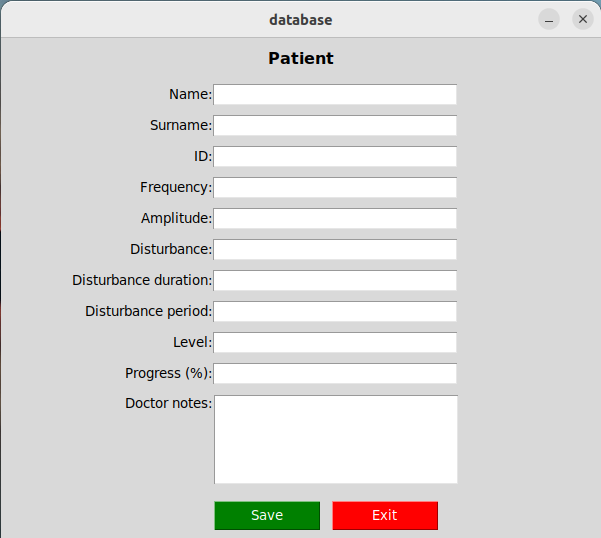
\includegraphics[width=\linewidth]{figs/registro.png}
	\end{minipage}
	\caption[Interfaz de registro de un paciente]{Interfaz de registro de un paciente}
	\label{fig:database}
\end{figure}

\section{Interfaz de control}



\section{Verbatim}

Para mencionar identificadores usados en el código ---como nombres de funciones o variables--- en el texto, usa el entorno literal o verbatim \verb|hypothesizeParallelograms()|. También se puede usar este entorno para varias líneas, como se ve a continuación:

\begin{verbatim}
void Memory::hypothesizeParallelograms () {
  // add your code here
}
\end{verbatim}

\section{Ecuaciones}

Si necesitas insertar alguna ecuación, puedes hacerlo. Al igual que las figuras, no te olvides de referenciarlas. A continuación se exponen algunas ecuaciones de ejemplo: Ecuación \ref{ec:ec1} y Ecuación \ref{ec:ec2}.

\begin{myequation}[h]
\begin{equation}
H = 1 - \frac{\sum_{i=0}^{N}\frac{(\frac{d_{j_s} + d_{j_e}}{2})}{N}}{M}
\nonumber
\label{ec:ec1}
\end{equation}
\caption[Ejemplo de ecuación con fracciones]{Ejemplo de ecuación con fracciones}
\end{myequation} 

\begin{myequation}[h]
\begin{equation}
v(entrada)= \left\{
	\begin{array}{lcc}
		0 & \mbox{if} & \epsilon_t < 0.1\\
		K_p\cdot{(T_{t}-T)} & \mbox{if}& 0.1 \leq \epsilon_t < M_t\\
		K_p \cdot M_t & \mbox{if}& M_t < \epsilon_t
	\end{array}
\right.
\label{ec:ec2}
\end{equation}
\caption[Ejemplo de ecuación con array y letras y símbolos especiales]{Ejemplo de ecuación con array y letras y símbolos especiales}
\end{myequation}

\section{Tablas o cuadros}

Si necesitas insertar una tabla, hazlo dígnamente usando las propias tablas de \LaTeX, no usando pantallazos e insertándolas como figuras... En el Cuadro \ref{cuadro:ejemplo} vemos un ejemplo.

\begin{table}[H]
\begin{center}
\begin{tabular}{|c|c|}
\hline
\textbf{Parámetros} & \textbf{Valores} \\
\hline
Tipo de sensor & Sony IMX219PQ[7] CMOS 8-Mpx \\
Tamaño del sensor & 3.674 x 2.760 mm (1/4" format) \\
Número de pixels & 3280 x 2464 (active pixels) \\
Tamaño de pixel & 1.12 x 1.12 um \\
Lente & f=3.04 mm, f/2.0 \\
Ángulo de visión & 62.2 x 48.8 degrees \\
Lente SLR equivalente & 29 mm \\
\hline
\end{tabular}
\caption{Parámetros intrínsecos de la cámara}
\label{cuadro:ejemplo}
\end{center}
\end{table}

